% Created 2025-06-21 Sat 22:50
% Intended LaTeX compiler: pdflatex
\documentclass[11pt]{report}
\usepackage[utf8]{inputenc}
\usepackage[T1]{fontenc}
\usepackage{graphicx}
\usepackage{grffile}
\usepackage{longtable}
\usepackage{wrapfig}
\usepackage{rotating}
\usepackage[normalem]{ulem}
\usepackage{amsmath}
\usepackage{textcomp}
\usepackage{amssymb}
\usepackage{capt-of}
\usepackage{hyperref}
\usepackage{minted}
\usepackage{adjustbox}
\author{John Russell}
\date{\today}
\title{Download Video\\\medskip
\large Easily download videos from Youtube and other sites.}
\hypersetup{
 pdfauthor={John Russell},
 pdftitle={Download Video},
 pdfkeywords={},
 pdfsubject={},
 pdfcreator={Emacs 27.1 (Org mode 9.3)},
 pdflang={English}}
\begin{document}

\maketitle
\tableofcontents

\begin{abstract}
Download Video is a commandline application for downloading videos from
Youtube and other sites.  The user can select a video format to download based
on one or more parameters, such as video height, whether to include audio,
et. al.
\end{abstract}

\part{Terminology}
\label{sec:org6e52071}

\begin{description}
\item[{Video}] In this document, refers to any video or audio file, including videos
with or without audio.
\item[{Site processor}] A singleton class that contains methods for handling
site-specific implementations of the \texttt{SiteProcessor} interface.
\end{description}

\part{User Interface}
\label{sec:org6668f97}

\chapter{{\bfseries\sffamily DONE} Main Application}
\label{sec:org224afe8}
\begin{itemize}
\item State "DONE"       from "TODO"       \textit{[2025-06-21 Sat 21:34]}
\end{itemize}
Download Video uses a CLI to interact with users.  The basic syntax is this:

\begin{verbatim}
Usage:
  download-video [-hny] URL
  download-video [-hny] [--height HEIGHT] [--video-only] URL
  download-video [-hny] [--audio-only] URL
  download-video [-hny] -r FILE
\end{verbatim}

The lone positional argument is treated as a string URL by default; if \textbf{-r} is
passed, it's treated as a path.

\textbf{Options}

\begin{center}
\begin{tabular}{lll}
Short & Long & Note\\
\hline
\texttt{-n} & \texttt{-{}-dry-run} & Prints only what will happen\\
\texttt{-r} & \texttt{-{}-rename} & Renames the file instead of downloading from \emph{URL}\\
 & \texttt{-{}-height} \emph{NUMBER} & Selects the best format according to the video height.\\
 & \texttt{-{}-audio-only} & Selects only audio formats\\
 & \texttt{-{}-video-only} & Selects only video formats\\
\texttt{-y} & \texttt{-{}-yes} & Automatically says yes to every prompt\\
\end{tabular}
\end{center}

\chapter{Config}
\label{sec:org160a58f}

This, shall we say, subcommand is derived from a submodule of the main package.
It has the following CLI:

\begin{verbatim}
Usage:
  download-video-config [-h] VARIABLE [VALUE]
\end{verbatim}

If \emph{VALUE} is provided, then \emph{VARIABLE} is set to that value.  Otherwise, the
current value of \emph{VARIABLE} is shown.

\part{Technical Specification}
\label{sec:org1850ec9}

\chapter{Dependencies}
\label{sec:orgbfeddb5}

Download Video uses:
\begin{description}
\item[{\href{https://pypi.org/project/typer}{typer}}] CLI
\item[{\href{https://pypi.org/project/yt-dlp}{yt-dlp}}] Backend
\item[{\href{https://pypi.org/project/pydantic}{pydantic}}] Validation of data, primarily the info dictionary
\end{description}

Standard library:
\begin{description}
\item[{\href{https://docs.python.org/3.12/library/urllib.parse.html}{\texttt{urllib.parse}}}] It conains \href{https://docs.python.org/3.12/library/urllib.parse.html\#urllib.parse.urlparse}{urlparse}, which we use to normalize URLs
\end{description}

\chapter{{\bfseries\sffamily TODO} Overview}
\label{sec:org3653058}
\begin{itemize}
\item State "DONE"       from "TODO"       \textit{[2025-06-21 Sat 21:31]}
\end{itemize}
\begin{figure}[htbp]
\centering
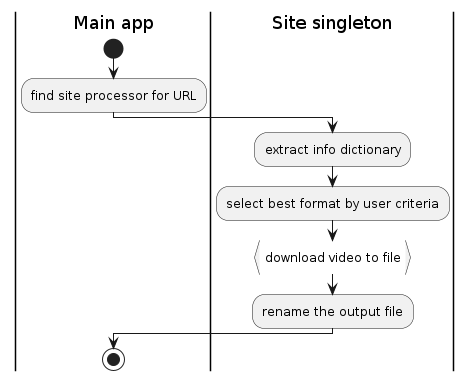
\includegraphics[width=.9\linewidth]{design-doc_files/act_overview.png}
\caption{Overview}
\end{figure}

\section{{\bfseries\sffamily DONE} Getting Site Processor}
\label{sec:orgb22400e}
\begin{itemize}
\item State "DONE"       from "TODO"       \textit{[2025-06-21 Sat 22:42]}
\end{itemize}
The URL is matched with a list of preregistered singletons known as \emph{site}
\emph{processors}.  That is to say, certain Python modules are treated as singletons.
When one of them matches with the URL, it is used for the remainder of the
process.

\begin{figure}[htbp]
\centering
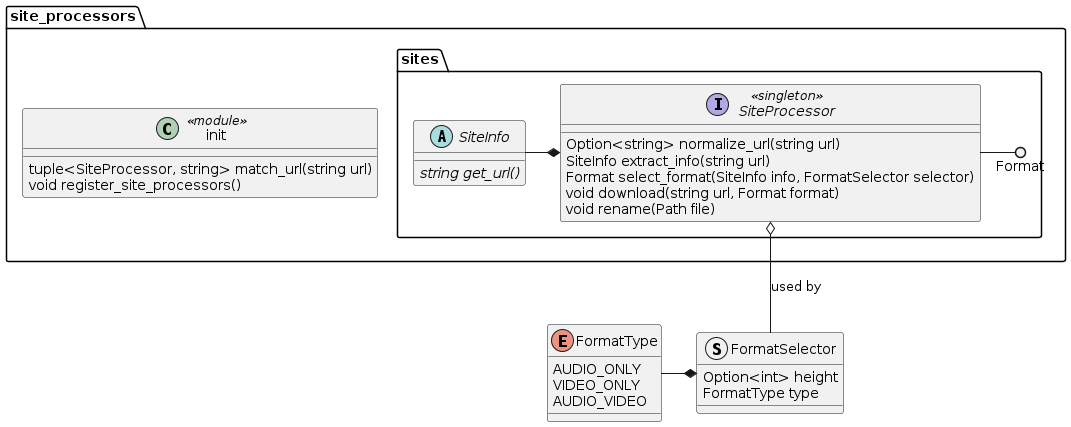
\includegraphics[width=.9\linewidth]{design-doc_files/cls_site-singleton.png}
\caption{\label{fig:org78b86b2}Site Processor}
\end{figure}

\section{{\bfseries\sffamily DONE} URL Normalization}
\label{sec:orge1fe2b1}
\begin{itemize}
\item State "DONE"       from "TODO"       \textit{[2025-06-21 Sat 22:48]}
\end{itemize}
The site processor has a function for normalizing URLs, which is done before
extracting the info dictionary.  The exact method will change depending on the
site processor (see \hyperref[sec:orgc697181]{Supported Sites}).

\section{{\bfseries\sffamily TODO} Extracting Info Dictionary}
\label{sec:org31486ab}
To extract an info dictionary, normally you would have to do this:

\begin{minted}[]{python}
params = {
    'clean_infojson': True,
    'restrictfilenames': True,
}
with YoutubeDL() as ydl:
    info = ydl.sanitize_info(ydl.extract_info(url, download=False))
\end{minted}

Now, this is done in the selected site processor.  Exactly what structure the
info dictionary has will depend on the site the URL belongs to.  A \texttt{SiteInfo}
object is returned to the caller, which then passes that \texttt{SiteInfo} to the next
step of the process.

\section{{\bfseries\sffamily TODO} Selecting A Format}
\label{sec:org7a43244}
The \texttt{select\_format} method selects a suitable format based on the criteria
provided by the user.  This criteria comes in the form of a \texttt{FormatSelector}
class.

The exact algorithm used for selecting a format depends on the site processor
used.  And the format itself is an opaque type (likely a string) whose exact
value we cannot know from the outside.  This is represented in Figure \ref{fig:org78b86b2}.

But in general, the following process is followed:
\begin{enumerate}
\item From the info dictionary, a list of formats is extracted.
\item The format list is filtered to only include audio and video formats,
including audio/video formats.
\item The format list is split three lists:
\begin{itemize}
\item A. Audio-only formats
\item B. Video-only formats
\item C. Audio/video formats
\end{itemize}
\item The format list is filtered using the strategy pattern.  See each supported
site for details.
\end{enumerate}

\begin{figure}[htbp]
\centering
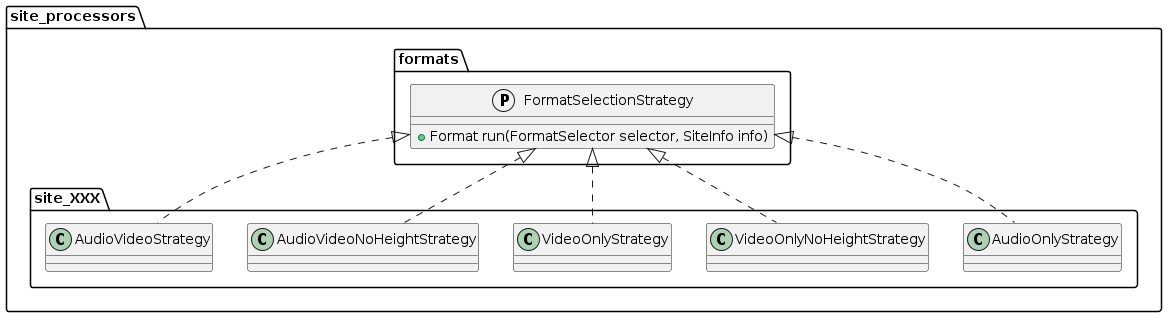
\includegraphics[width=.9\linewidth]{design-doc_files/cls_format-selection.png}
\caption{Format Selections}
\end{figure}

\chapter{Configuration}
\label{sec:orgd184da9}

A configuration file controls the exact behavior of Download Video.  There is a
global section followed sections for each supported site.  Their respective
values are explained under \hyperref[sec:orgc697181]{Supported Sites}.

The \texttt{config} subpackage handles the entire configuration framework.  In the
standard config directory, a Toml file is used called \texttt{config.toml}.

\chapter{Supported Sites}
\label{sec:orgc697181}

\section{{\bfseries\sffamily TODO} Youtube}
\label{sec:org682ea1f}
Right now, Youtube is the only site supported by Download Video.  This will likely
change in the future when this project has taken shape and is out of alpha.

The site processor for Youtube matches URLs with the following formats:
\begin{itemize}
\item https​://www.youtube.com/watch?v=XXXXXXXXXXX
\item youtu.be/XXXXXXXXXXX
\item yt:XXXXXXXXXXX
\end{itemize}

This site processor normalizes the URL so that it always has the first form.
The info dictionary returned by Youtube has this structure:

\begin{figure}[htbp]
\centering
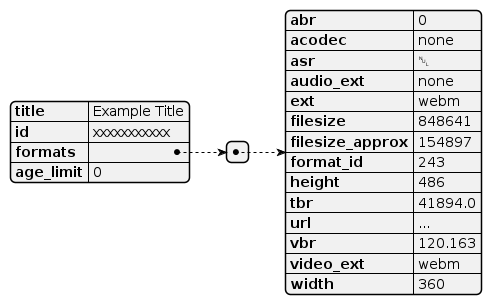
\includegraphics[width=.9\linewidth]{design-doc_files/dig_youtube-json.png}
\caption{Info Dictionary - Youtube}
\end{figure}

\begin{enumerate}
\item {\bfseries\sffamily TODO} URL Normalization
\label{sec:org8844177}
URL normalization is done by matching a URL with a regular expression and
capturing the video ID, then returning a "proper" URL with said video ID.

\item {\bfseries\sffamily TODO} Format Selection
\label{sec:org4edc29a}
Selecting a format is done by trying to get the best (highest quality) video
which satisfies the criteria outlined in \texttt{FormatSelector} (see Figure \ref{fig:org78b86b2}).

\begin{figure}[htbp]
\centering
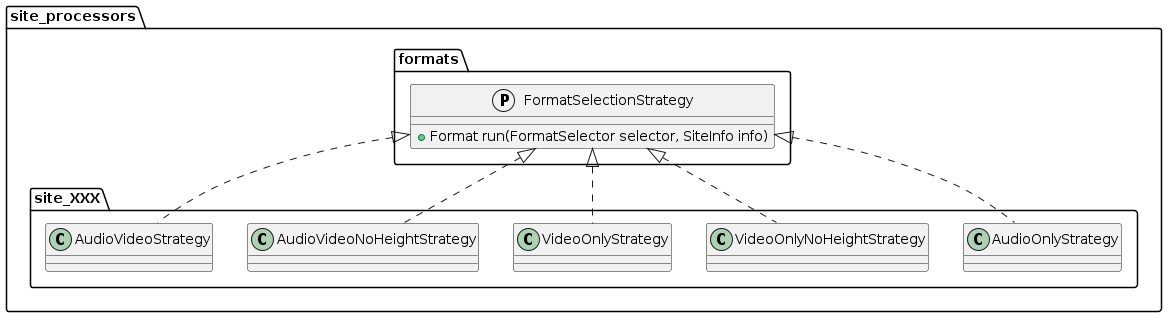
\includegraphics[width=.9\linewidth]{design-doc_files/cls_format-selection.png}
\caption{Format Selections}
\end{figure}

A series of strategies are used to filter the list formats according to the
criteria given.  The name of each strategy class pretty much says what the
strategy will be.  Then the highest quality format is chosen.  The barometer for
a format's quality is its total bitrate, denoted in the \texttt{tbr} element.
\end{enumerate}
\end{document}
